%%%%%%%%%%%%%%%%%%%%%%%%%%%%%%%%%%%%%%%%%%%%%%%%%%%%%%%%%%%%%%%%%%%%%%%%%%
%
% Plantilla para libro de texto de matemáticas.
%
% Esta plantilla ha sido desarrollada desde cero, pero utiliza algunas partes
% del código de la plantilla original utilizada en apuntesDGIIM
% (https://github.com/libreim/apuntesDGIIM), basada a su vez en las plantillas
% 'Short Sectioned Assignment' de Frits Wenneker (http://www.howtotex.com),
% 'Plantilla de Trabajo' de Mario Román y 'Plantilla básica de Latex en Español'
% de Andrés Herrera Poyatos (https://github.com/andreshp). También recoge
% ideas de la plantilla 'Multi-Purpose Large Font Title Page' de
% Frits Wenneker y Vel (vel@latextemplates.com).
%
% Licencia:	
% CC BY-NC-SA 4.0 (https://creativecommons.org/licenses/by-nc-sa/4.0/)
%
%%%%%%%%%%%%%%%%%%%%%%%%%%%%%%%%%%%%%%%%%%%%%%%%%%%%%%%%%%%%%%%%%%%%%%%%%

% ---------------------------------------------------------------------------
% CONFIGURACIÓN BÁSICA DEL DOCUMENTO
% ---------------------------------------------------------------------------

%\documentclass[11pt, a4paper, twoside]{article} % Usar para imprimir
\documentclass[10pt, a4paper]{article}

\linespread{1.3}            % Espaciado entre líneas.
\setlength\parindent{0pt}   % No indentar el texto por defecto.
\setlength\parskip{7pt}

% ---------------------------------------------------------------------------
% PAQUETES BÁSICOS
% ---------------------------------------------------------------------------

% IDIOMA
\usepackage[utf8]{inputenc}
\usepackage[spanish, es-tabla, es-lcroman, es-noquoting]{babel}
\usepackage[table,xcdraw]{xcolor}

% MATEMÁTICAS
\usepackage{amsmath}    % Paquete básico de matemáticas
\usepackage{amsthm}     % Teoremas
\usepackage{mathrsfs}   % Fuente para ciertas letras utilizadas en matemáticas

% FUENTES
\usepackage{newpxtext, newpxmath}   % Fuente similar a Palatino
\usepackage{FiraSans}                 % Fuente sans serif
\usepackage[T1]{fontenc}
\usepackage[italic]{mathastext}     % Utiliza la fuente del documento
                                    % en los entornos matemáticos

% MÁRGENES
\usepackage[margin=2.5cm, top=3cm]{geometry}

% LISTAS
\usepackage{enumitem}       % Mejores listas
\setlist{leftmargin=.5in}   % Especifica la indentación para las listas.

% Listas ordenadas con números romanos (i), (ii), etc.
\newenvironment{nlist}
{\begin{enumerate}
    \renewcommand\labelenumi{(\emph{\roman{enumi})}}}
  {\end{enumerate}}

%  OTROS
\usepackage[hidelinks]{hyperref}   % Enlaces
\usepackage{graphicx}   % Permite incluir gráficos en el documento
\usepackage{relsize}

% LISTINGS
\usepackage{listings}
\usepackage{xcolor}     % Permite definir y utilizar colores
\usepackage{lipsum}
\usepackage{courier}

% Fijar tabla a posición
\usepackage{array}
\newcolumntype{L}[1]{>{\raggedright\let\newline\\\arraybackslash\hspace{0pt}}m{#1}}
\newcolumntype{C}[1]{>{\centering\let\newline\\\arraybackslash\hspace{0pt}}m{#1}}
\newcolumntype{R}[1]{>{\raggedleft\let\newline\\\arraybackslash\hspace{0pt}}m{#1}}


% Colores para los bloques de código
\definecolor{codegreen}{rgb}{0,0.6,0}
\definecolor{codegray}{rgb}{0.5,0.5,0.5}
\definecolor{codepurple}{rgb}{0.58,0,0.82}
\definecolor{backcolour}{rgb}{0.95,0.95,0.92}
\lstdefinestyle{mystyle}{
	backgroundcolor=\color{backcolour},   
	commentstyle=\color{codegreen},
	keywordstyle=\color{blue},
	numberstyle=\tiny\color{codegray},
	stringstyle=\color{codepurple},
	basicstyle=\footnotesize\ttfamily,
	breakatwhitespace=false,         
	breaklines=true,                 
	captionpos=b,                    
	keepspaces=true,                 
	numbers=left,                    
	numbersep=5pt,                  
	showspaces=false,                
	showstringspaces=false,
	showtabs=false,                  
	tabsize=4
}
\lstset{style=mystyle}

%\lstset{basicstyle=\footnotesize\ttfamily,breaklines=true}
%\lstset{framextopmargin=50pt,frame=bottomline}
 
% ---------------------------------------------------------------------------
% COMANDOS PERSONALIZADOS
% ---------------------------------------------------------------------------

% \equalto
\newcommand{\verteq}{\rotatebox{90}{$\,=$}}
\newcommand{\equalto}[2]{\underset{\scriptstyle\overset{\mkern4mu\verteq}{#2}}{#1}}


% ---------------------------------------------------------------------------
% COLORES
% ---------------------------------------------------------------------------

\definecolor{50}{HTML}{E0F2F1}
\definecolor{100}{HTML}{B2DFDB}
\definecolor{200}{HTML}{80CBC4}
\definecolor{300}{HTML}{4DB6AC}
\definecolor{400}{HTML}{26A69A}
\definecolor{500}{HTML}{009688}
\definecolor{600}{HTML}{00897B}
\definecolor{700}{HTML}{00796B}
\definecolor{800}{HTML}{00695C}
\definecolor{900}{HTML}{004D40}

% ---------------------------------------------------------------------------
% DISEÑO DE PÁGINA
% ---------------------------------------------------------------------------

\usepackage{pagecolor}
\usepackage{afterpage}

% ---------------------------------------------------------------------------
% CABECERA Y PIE DE PÁGINA
% ---------------------------------------------------------------------------

\usepackage{fancyhdr}   % Paquete para cabeceras y pies de página

% Indica que las páginas usarán la configuración de fancyhdr
\pagestyle{fancy}
\fancyhf{}

% Representa la sección de la cabecera
\renewcommand{\sectionmark}[1]{%
\markboth{#1}{}}

% Representa la subsección de la cabecera
\renewcommand{\subsectionmark}[1]{%
\markright{#1}{}}

% Parte derecha de la cabecera
\fancyhead[LE,RO]{\sffamily\textsl{\rightmark} \hspace{1em}  \textcolor{500}{\rule[-0.4ex]{0.2ex}{1.2em}} \hspace{1em} \thepage}

% Parte izquierda de la cabecera
\fancyhead[RE,LO]{\sffamily{\leftmark}}

% Elimina la línea de la cabecera
\renewcommand{\headrulewidth}{0pt}

% Controla la altura de la cabecera para que no haya errores
\setlength{\headheight}{14pt}

% ---------------------------------------------------------------------------
% TÍTULOS DE PARTES Y SECCIONES
% ---------------------------------------------------------------------------

\usepackage{titlesec}

% Estilo de los títulos de las partes
\titleformat{\part}[hang]{\Huge\bfseries\sffamily}{\thepart\hspace{20pt}\textcolor{500}{|}\hspace{20pt}}{0pt}{\Huge\bfseries}
\titlespacing*{\part}{0cm}{-2em}{2em}[0pt]

% Reiniciamos el contador de secciones entre partes (opcional)
\makeatletter
\@addtoreset{section}{part}
\makeatother

% Estilo de los títulos de las secciones, subsecciones y subsubsecciones
\titleformat{\section}
  {\Large\bfseries\sffamily}{\thesection}{1em}{}

\titleformat{\subsection}
  {\Large\sffamily}{\thesubsection}{1em}{}[\vspace{.5em}]

\titleformat{\subsubsection}
  {\sffamily}{\thesubsubsection}{1em}{}

% ---------------------------------------------------------------------------
% ENTORNOS PERSONALIZADOS
% ---------------------------------------------------------------------------

\usepackage{mdframed}

%% DEFINICIONES DE LOS ESTILOS

% Nuevo estilo para definiciones
\newtheoremstyle{definition-style}  % Nombre del estilo
{}                                  % Espacio por encima
{}                                  % Espacio por debajo
{}                                  % Fuente del cuerpo
{}                                  % Identación
{\bf\sffamily}                      % Fuente para la cabecera
{.}                                 % Puntuación tras la cabecera
{.5em}                              % Espacio tras la cabecera
{\thmname{#1}\thmnumber{ #2}\thmnote{ (#3)}}  % Especificación de la cabecera

% Nuevo estilo para notas
\newtheoremstyle{remark-style}
{10pt}
{10pt}
{}
{}
{\itshape \sffamily}
{.}
{.5em}
{}

% Nuevo estilo para teoremas y proposiciones
\newtheoremstyle{theorem-style}
{}
{}
{}
{}
{\bfseries \sffamily}
{.}
{.5em}
{\thmname{#1}\thmnumber{ #2}\thmnote{ (#3)}}

% Nuevo estilo para ejemplos
\newtheoremstyle{example-style}
{10pt}
{10pt}
{}
{}
{\bf \sffamily}
{}
{.5em}
{\thmname{#1}\thmnumber{ #2.}\thmnote{ #3.}}

% Nuevo estilo para la demostración

\makeatletter
\renewenvironment{proof}[1][\proofname] {\par\pushQED{\qed}\normalfont\topsep6\p@\@plus6\p@\relax\trivlist\item[\hskip\labelsep\itshape\sffamily#1\@addpunct{.}]\ignorespaces}{\popQED\endtrivlist\@endpefalse}
\makeatother

%% ASIGNACIÓN DE LOS ESTILOS

% Teoremas, proposiciones y corolarios
\newtheoremstyle{theorem-style}{}{}{}{}{}{}{ }{}
\theoremstyle{theorem-style}
\newtheorem*{datos}{}
\theoremstyle{theorem-style}
\newtheorem{nth}{Teorema}[section]
\newtheorem{nprop}{Proposición}[section]
\newtheorem{ncor}{Corolario}[section]
\newtheorem{lema}{Lema}[section]

% Definiciones
\theoremstyle{definition-style}
\newtheorem{ndef}{Definición}[section]

% Notas
\theoremstyle{remark-style}
\newtheorem*{nota}{Nota}

% Ejemplos
\theoremstyle{example-style}
\newtheorem{ejemplo}{Ejemplo}[section]

% Ejercicios y solución
\theoremstyle{definition-style}
\newtheorem{ejer}{Ejercicio}[section]

\theoremstyle{remark-style}
\newtheorem*{sol}{Solución}

%% MARCOS DE LOS ESTILOS

% Configuración general de mdframe, los estilos de los teoremas, etc
\mdfsetup{
  skipabove=1em,
  skipbelow=1em,
  innertopmargin=1em,
  innerbottommargin=1em,
  splittopskip=2\topsep,
}

% Definimos los marcos de los estilos


\mdfdefinestyle{datos-frame}{
	linewidth=2pt, %
	linecolor= 500, %
	topline=false, %
	bottomline=false, %
	rightline=false,%
	leftmargin=0em, %
	innerleftmargin=1em, %
	innerrightmargin=1em,
	rightmargin=0em, %
}%
\mdfdefinestyle{nth-frame}{
	linewidth=2pt, %
	linecolor= 500, %
	topline=false, %
	bottomline=false, %
	rightline=false,%
	leftmargin=0em, %
	innerleftmargin=1em, %
  innerrightmargin=1em,
	rightmargin=0em, %
}%

\mdfdefinestyle{nprop-frame}{
	linewidth=2pt, %
	linecolor= 300, %
	topline=false, %
	bottomline=false, %
	rightline=false,%
	leftmargin=0pt, %
	innerleftmargin=1em, %
	innerrightmargin=1em,
	rightmargin=0pt, %
}%

\mdfdefinestyle{ndef-frame}{
	linewidth=2pt, %
	linecolor= 500, %
	backgroundcolor= 50,
	topline=false, %
	bottomline=false, %
	rightline=false,%
	leftmargin=0pt, %
	innerleftmargin=1em, %
	innerrightmargin=1em,
	rightmargin=0pt, %
}%

\mdfdefinestyle{ejer-frame}{
	linewidth=2pt, %
	linecolor= 300, %
	backgroundcolor= 50,
	topline=false, %
	bottomline=false, %
	rightline=false,%
	leftmargin=0pt, %
	innerleftmargin=1em, %
	innerrightmargin=1em,
	rightmargin=0pt, %
}%

\mdfdefinestyle{ejemplo-frame}{
	linewidth=0pt, %
	linecolor= 300, %
	leftline=false, %
	rightline=false, %
	leftmargin=0pt, %
	innerleftmargin=1.3em, %
	innerrightmargin=1em,
	rightmargin=0pt, %
	innertopmargin=0em,%
	innerbottommargin=0em, %
	splittopskip=\topskip, %
}%

% Asignamos los marcos a los estilos
\surroundwithmdframed[style=nth-frame]{nth}
\surroundwithmdframed[style=datos-frame]{datos}
\surroundwithmdframed[style=nprop-frame]{nprop}
\surroundwithmdframed[style=nprop-frame]{ncor}
\surroundwithmdframed[style=ndef-frame]{ndef}
\surroundwithmdframed[style=ejer-frame]{ejer}
\surroundwithmdframed[style=ejemplo-frame]{ejemplo}
\surroundwithmdframed[style=ejemplo-frame]{sol}

% ---------------------------------------------------------------------------
% CONFIGURACIÓN DE LA PORTADA
% ---------------------------------------------------------------------------

\newcommand{\asignatura}{Análisis de eficiencia de algoritmos}

\newcommand{\autor}{Celia Arias Martínez\\Miguel Ángel Fernández Gutiérrez\\Sergio Quijano Rey\\Lucía Salamanca López\\\hspace{1cm}}

\newcommand{\grado}{segfault}

\newcommand{\universidad}{Universidad de Granada}

\newcommand{\enlaceweb}{github.com/DGIIMUnderground}

% ---------------------------------------------------------------------------
% CONFIGURACIÓN PERSONALIZADA
% ---------------------------------------------------------------------------

%%%%%%%%%%%%%%%%%%%%%%%%%%%%%%%%%%%%%%%%%%%%%%%%%%%%%%%%%%%%%%%%%%%%%%%%%%%%%
% ---------------------------------------------------------------------------
% COMIENZO DEL DOCUMENTO
% ---------------------------------------------------------------------------
%%%%%%%%%%%%%%%%%%%%%%%%%%%%%%%%%%%%%%%%%%%%%%%%%%%%%%%%%%%%%%%%%%%%%%%%%%%%%

\begin{document}

% ---------------------------------------------------------------------------
% PORTADA EXTERIOR
% ---------------------------------------------------------------------------

\newpagecolor{500}\afterpage{\restorepagecolor} % Color de la página
\begin{titlepage}

  % Título del documento
	\parbox[t]{\textwidth}{
			\raggedright % Texto alineado a la izquierda
			\fontsize{40pt}{40pt}\selectfont\sffamily\color{white}{
				\textbf{\Huge{Práctica 3}}\\\textbf{Algoritmos voraces (\emph{greedy})}\\\huge{Algorítmica}
      }
	}

	\vfill

	%% Autor e información del documento
	\parbox[t]{\textwidth}{
		\raggedright % Texto alineado a la izquierda
		\sffamily\large\color{white}
		\grado\\
		{\Large \autor }\\[15pt]
		
\includegraphics[width=130pt]{ugrlogo.pdf}
	}

\end{titlepage}

% ---------------------------------------------------------------------------
% PÁGINA DE LICENCIA
% ---------------------------------------------------------------------------

\thispagestyle{empty}
\null
\vfill

%% Información sobre la licencia
\parbox[t]{\textwidth}{
  
\includegraphics{by-nc-sa.pdf}\\[4pt]
  \raggedright % Texto alineado a la izquierda
  \sffamily\large
  {\Large Este trabajo se distribuye bajo una licencia CC BY-NC-SA 4.0.}\\[4pt]
  Eres libre de distribuir y adaptar el material siempre que reconozcas a los\\
  autores originales del documento, no lo utilices para fines comerciales\\
  y lo distribuyas bajo la misma licencia.\\[4pt]
  \texttt{creativecommons.org/licenses/by-nc-sa/4.0/}
}

% ---------------------------------------------------------------------------
% PORTADA INTERIOR
% ---------------------------------------------------------------------------

\begin{titlepage}

  % Título del documento
  \parbox[t]{\textwidth}{
  	\raggedright % Texto alineado a la izquierda
  	\fontsize{40pt}{40pt}\selectfont\sffamily\color{500}{
  		\textbf{\Huge{Práctica 3}}\\\textbf{Algoritmos voraces (\emph{greedy})}\\\huge{Algorítmica}
  	}
  }

	\vfill
	
	%% Autor e información del documento
	\parbox[t]{\textwidth}{
		\raggedright % Texto alineado a la izquierda
		\sffamily\large
		\grado\\
		{\Large \autor }\\[15pt]
		
\includegraphics[width=130pt]{ugrlogo-dark.pdf}
	}

\end{titlepage}

% ---------------------------------------------------------------------------
% ÍNDICE
% ---------------------------------------------------------------------------

\thispagestyle{empty}
\tableofcontents
\newpage

% ---------------------------------------------------------------------------
% CONTENIDO
% ---------------------------------------------------------------------------

\part{Introducción}

Esta \textbf{práctica 3}, de desarrollo de algoritmos \emph{greedy}, consiste en dos partes principales:

\begin{itemize}
	\item \textbf{Problema común:} problema del viajante de comercio.
	\item \textbf{Problema asignado:} asignación de tareas.
\end{itemize}

\subsection*{Objetivo de esta práctica}

En esta práctica, pretenderemos apreciar la utilidad de los algoritmos voraces (\emph{greedy}) para la resolución de problemas de forma eficiente, en algunos casos obteniendo soluciones óptimas y en otros aproximaciones.

Para ello, daremos diversas soluciones \emph{greedy} a los problemas asignados, y compararemos la bondad en la solución y la eficiencia de estos algoritmos, dando especial importancia al uso de \textbf{permutaciones} para acercarnos a soluciones cada vez mejores con sucesivas iteraciones, como veremos en los últimos enfoques de cada problema (\emph{sección II, apartados 1.3} y \emph{2.2}).

\pagebreak
\part{Desarrollo}

A continuación, estudiaremos los dos algoritmos propuestos.

\section{Problema del viajante de comercio (TSP)}

\begin{datos}
	{\sffamily Dado un conjunto de ciudades y una matriz con las distancias entre ellas, buscar el recorrido mínimo que que pase por todas ellas una vez y vuelva al punto de partida.
	
	Formalmente: dado un grafo \emph{G}, conexo y ponderado, se trata de hallar el \emph{ciclo hamiltoniano} de mínimo peso de ese grafo.}
\end{datos}

\subsection*{Elementos comunes}

A lo largo de la solución del problema usaremos la siguiente notación:

\begin{itemize}
	\item $n$ es el \textbf{número de ciudades}.
	\item $D$ es la \textbf{matriz de distancias}.
	\item $r$ es el \textbf{vector de recorrido}, que contiene un itinerario que pasa por todas las ciudades, es decir, $n$ elementos no repetidos.
	\item $W_r$ es el \textbf{coste} de un recorrido, es decir, la distancia de un recorrido $r$.
\end{itemize}

\subsection{Enfoque por cercanía}

Este algoritmo \emph{greedy} es muy simple:

\begin{enumerate}
	\item Partimos de un nodo cualquiera.
	\item Encontramos el nodo más cercano a este nodo, y lo añadimos al recorrido.
	\item Repetimos el proceso hasta cubir todos los nodos (encontrando el siguiente nodo más cercano).
	\item Añadimos el nodo de vuelta.
\end{enumerate}

Hacemos uso del siguiente código:

\begin{lstlisting}[language=C]
vector<common::Point> get_best_solution(vector<common::Point> points){
	vector<common::Point> road;                 // Solucion que vamos a construir
	vector<common::Point> points_left = points; // Puntos que quedan por insertar a la solucion
	// Parto siempre del primer punto del vector
	road.push_back(points_left[0]);
	points_left.erase(points_left.begin() + 0);
	// Voy construyendo la solucion, sacando puntos de points_left y colocandolos en road
	while(points_left.size() > 0){
		double min_distance = common::distance(road[road.size() -1], points_left[0]);
		int min_pos = 0;
		// Buscamos el punto mas cercano
		for(int i = 0; i < points_left.size(); i++){
			double current_distance = common::distance(road[road.size() -1], points_left[i]);
			if(current_distance < min_distance){
				min_distance = current_distance;
				min_pos = i;
		}
	}
	// Insertamos el punto mas cercano a la solucion y lo quitamos de los puntos que faltan
	road.push_back(points_left[min_pos]);
	points_left.erase(points_left.begin() + min_pos);
	}
	return road;
}
\end{lstlisting}

En el que utilizamos las siguientes funciones y estructuras de datos:

\begin{itemize}
	\item Un \emph{struct} \texttt{Point}, que tiene una coordenada \texttt{x}, una coordenada \texttt{y}, y una función \texttt{distancia} para calcular la distancia entre dos \texttt{Point}.
	\item Una función \texttt{get\_best\_solution}, que calcula la solución especificada anteriormente. Para ello, hace uso de:
	\begin{itemize}
		\item \texttt{road}, un vector donde se almacenan las soluciones parciales, es decir, las que resultan de añadir un nodo al recorrido.
		\item \texttt{points\_left}, vector donde almacenamos los nodos que nos quedan por recorrer.
	\end{itemize}
	\item[] Guardamos en \texttt{points\_left} todos los nodos y en \texttt{road} el primer punto, que podemos asumir que es el primero. 
Mientras que el vector \texttt{points\_left} no esté vacío calculamos la distancia de todos esos nodos al último Punto de \texttt{road} y añadimos el nodo que esté a la menor distancia, borrándolo de \texttt{points\_left}.
\end{itemize}
El código completo se encuentra en la \textbf{\emph{sección IV: Anexo I}} de este documento.

\subsubsection*{Análisis empírico}

Los tamaños de prueba para ejecutar el algoritmo han ido desde 100 hasta 4000 ciudades, cada vez con incremento de 200. A su vez cada iteración la hemos hecho 100 veces y hemos calculado la media, con el fin de eliminar los mejores y peores casos.

\pagebreak

Los datos obtenidos, calculando por un lado el tiempo y por otro la distancia han sido estos:

\begin{datos}
	{\bf\sffamily Gráfico 1.1.1.} {\sffamily Datos empíricos para viajante de comercio versión cercanía, tiempo}\\
	\vspace{-0.7cm}
	\begin{center}
		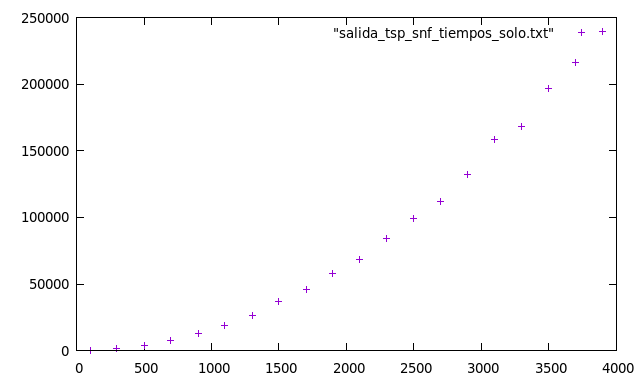
\includegraphics[width=15cm]{./../Graficas/graficastsp/snfTiempo.png}
	\end{center}	
\end{datos}

\begin{datos}
	{\bf\sffamily Gráfico 1.1.2.} {\sffamily Datos empíricos para viajante de comercio versión cercanía, distancia.}\\
	\vspace{-0.7cm}
	\begin{center}
		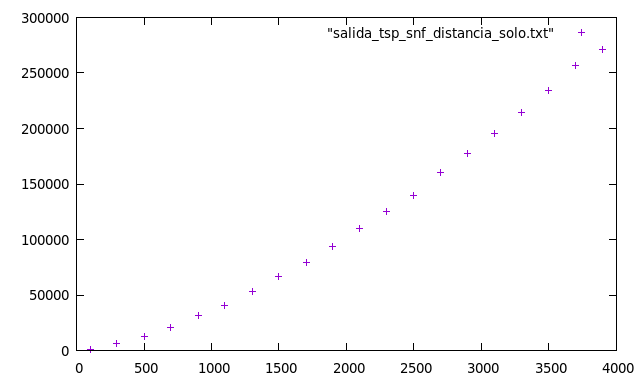
\includegraphics[width=15cm]{./../Graficas/graficastsp/snfDistancia.png}
	\end{center}	
\end{datos}

Los datos de las gráficas se encuentran en la \textbf{\emph{sección IV: Anexo II}} de este documento.

\subsection{Enfoque por inserción}

Este algoritmo \emph{greedy} funciona tomando un recorrido dado e insertando nodos de modo que el recorrido sea mínimo.

\begin{lstlisting}[language=C]
vector<common::Point> get_best_solution(vector<common::Point> points){
	vector<common::Point> candidates = points;  // Vector con los candidatos
	vector<common::Point> road;                 // Vector con la solucion parcial
	
	// Tomo los tres puntos extremos del plano y los coloco como solucion parcial inicial
	int most_north = get_most_north(candidates);
	int most_east = get_most_east(candidates);
	int most_west = get_most_west(candidates);
	
	road.push_back(candidates[most_north]);
	road.push_back(candidates[most_west]);
	road.push_back(candidates[most_east]);
	
	candidates.erase(candidates.begin() + most_north);
	candidates.erase(candidates.begin() + most_west);
	candidates.erase(candidates.begin() + most_east);
	
	// Construyo las soluciones parciales
	while(candidates.size() > 0){
		// Tomo el mejor candidato para la siguiente iteracion
		vector<int> best_candidate_and_pos = get_best_candidate(road, candidates);
		int best_candidate = best_candidate_and_pos[0];
		int best_pos = best_candidate_and_pos[1];
		
		// Hago el traspase de candidatos a solucion parcial
		road.insert(road.begin() + best_pos, candidates[best_candidate]);
		candidates.erase(candidates.begin() + best_candidate);
	}
	
	return road;
}
\end{lstlisting}

En este código, tenemos que:
\begin{itemize}
	\item \texttt{candidates} es el vector con los nodos que faltan por insertar. 
	\item \texttt{road} es el vector con la solución parcial. 
	\item \texttt{most\_north} es el nodo más al norte.
	\item \texttt{most\_west} es el nodo más al oeste.
	\item \texttt{most\_east} es el nodo más al este.
	\item \texttt{get\_best\_candidate} es una función auxiliar que dado un camino y un vector de candidatos devuelve un vector con la posición del punto óptimo y dónde queremos insertarlo en el camino. 
\end{itemize}

En la nueva función \texttt{get\_best\_solution}, primero calculamos e insertamos en \texttt{road} los nodos más al norte, este y oeste, para que se queden dentro los máximos nodos posibles. Mientras que \texttt{candidates} no sea vacío calculamos el nodo y la posición con los cuales la distancia que tenemos que recorrer aumenta lo mínimo posible al añadir un nodo, y lo insertamos en \texttt{road}, quitándolo de \texttt{candidates}.

\subsubsection*{Análisis empírico}

Los tamaños de prueba para ejecutar el algoritmo han ido desde 3 hasta 200 ciudades, cada vez con incremento de 10. A su vez cada iteración la hemos hecho 100 veces y hemos calculado la media, con el fin de eliminar los mejores y peores casos.  

Los datos obtenidos, calculando por un lado el tiempo y por otro la distancia han sido estos:

\begin{datos}
	{\bf\sffamily Gráfico 1.2.1.} {\sffamily Datos empíricos para viajante de comercio versión inserción, tiempo}\\
	\vspace{-0.7cm}
	\begin{center}
		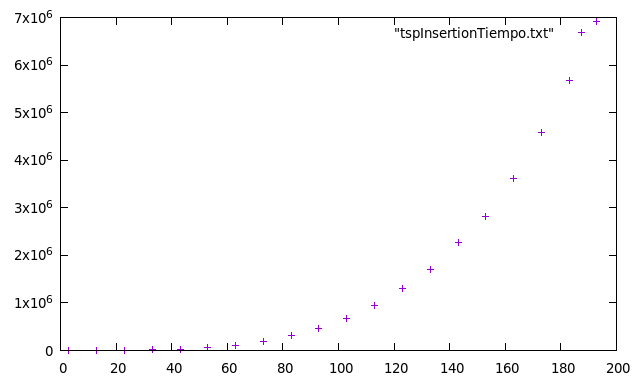
\includegraphics[width=15cm]{../Graficas/graficastsp/insertionTiempo.png}
	\end{center}	
\end{datos}

\pagebreak

\begin{datos}
	{\bf\sffamily Gráfico 1.2.2.} {\sffamily Datos empíricos para viajante de comercio versión inserción, distancia}\\
	\vspace{-0.7cm}
	\begin{center}
		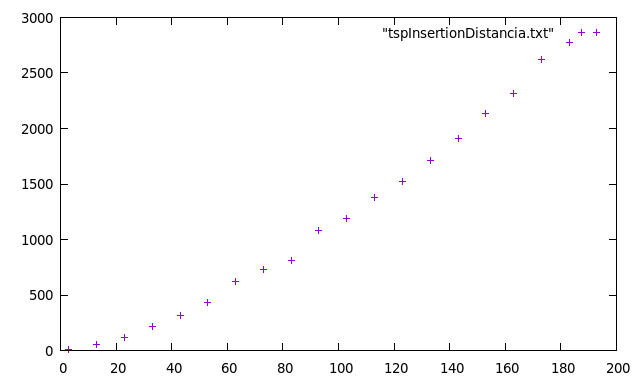
\includegraphics[width=15cm]{../Graficas/graficastsp/insertionDistancia.png}
	\end{center}	
\end{datos}

Los datos de las gráficas se encuentran en la \textbf{\emph{sección IV: Anexo II}} de este documento.

\subsection{Enfoque por perturbaciones}

Este enfoque, de nuevo \emph{greedy}, dado un recorrido, realiza las perturbaciones indicadas por un parámetro para intentar mejorarlo.

\begin{lstlisting}[language=C]
vector<common::Point> get_best_solution(vector<common::Point> points, int perturbations){
	// Tomo la solucion dada por el snf
	vector<common::Point> base_road = get_snf_solution(points);
	
	// Perturbo el numero de veces indicada
	for(int i = 0; i < perturbations; i++){
		// Calculo la posicion respecto a la que perturbar
		int pos = get_worst_node(points);
		
		// Perturbo el camino base
		perturbate(base_road, pos);
	}
	
	return base_road;
}
\end{lstlisting}

En este código, tenemos que:
\begin{itemize}
	\item \texttt{points} es un vector con los nodos dados. 
	\item \texttt{perturbations} es el número de perturbaciones que aplicamos al algoritmo. 
	\item \texttt{get\_snf\_solution} es una función auxiliar que calcula según el algoritmo por cercanía una solución al conjunto de puntos.
	\item \texttt{get\_worst\_node} es una función auxiliar que calcula el nodo tal que según el recorrido actual su distancia al siguiente punto es la mayor.
	\item \texttt{perturbate} es una función auxiliar que encuentra un camino diferente que haga que el peor nodo mejore y sobrescribe el camino actual.
\end{itemize}

Primero calculamos una solución inicial con el algoritmo de \emph{cercanía}. Después calculamos el peor nodo de ese recorrido e intentamos encontrar otra combinación de nodos que mejore ese nodo en concreto. Este proceso lo repetimos tantas veces como \texttt{perturbations} indique. 

\subsubsection*{Análisis empírico}

Los tamaños de prueba para ejecutar el algoritmo han ido desde 10 hasta 200 ciudades, cada vez con incremento de 20. A su vez cada iteración la hemos hecho 100 veces y hemos calculado la media, con el fin de eliminar los mejores y peores casos.  

Los datos obtenidos, calculando por un lado el tiempo y por otro la distancia han sido estos:

\begin{datos}
	{\bf\sffamily Gráfico 1.3.1.} {\sffamily  Datos empíricos para viajante de comercio versión perturbaciones, tiempo}\\
	\vspace{-0.7cm}
	\begin{center}
		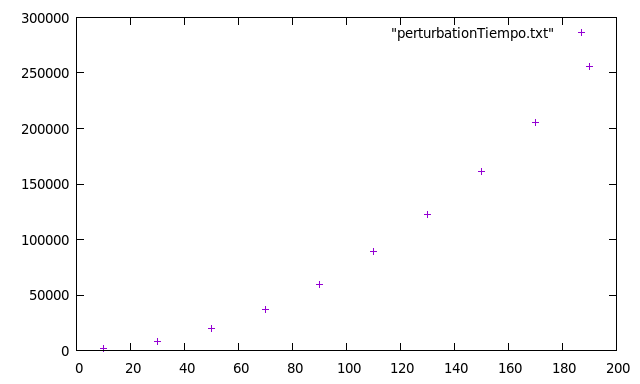
\includegraphics[width=15cm]{../Graficas/graficastsp/perturbationTiempo.png}
	\end{center}	
\end{datos}

\pagebreak

\begin{datos}
	{\bf\sffamily Gráfico 1.3.2.} {\sffamily Datos empíricos para viajante de comercio versión perturbaciones, distancia}\\
	\vspace{-0.7cm}
	\begin{center}
		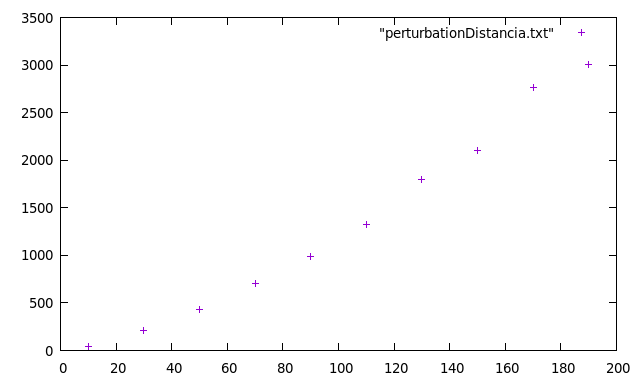
\includegraphics[width=15cm]{../Graficas/graficastsp/perturbationDistancia.png}
	\end{center}	
\end{datos}

Los datos de las gráficas se encuentran en la \textbf{\emph{sección IV: Anexo II}} de este documento.

\pagebreak

\subsection{Comparación de enfoques}

Los cuatro algoritmos que tenemos son: cercanía, inserción, fuerza bruta y perturbaciones. \\
Vamos a comparar por separado las gráficas de las distancias y los tiempos de los tres primeros algoritmos. Como el algoritmo de fuerza bruta solo funciona para tamaños muy pequeños pondremos la cota en 10 nodos.


\begin{datos}
	{\bf\sffamily Gráfico 1.4.1.} {\sffamily Contraste de datos empíricos: tiempo}\\
	\vspace{-0.7cm}
	\begin{center}
		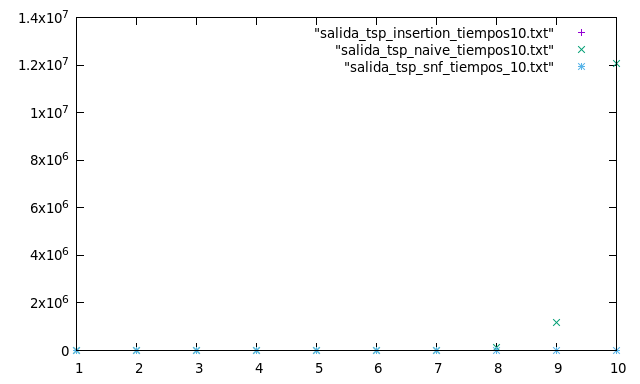
\includegraphics[width=15cm]{../Graficas/graficastsp/tiempo3.png}
	\end{center}	
\end{datos}
\pagebreak
\begin{datos}
	{\bf\sffamily Gráfico 1.4.2.} {\sffamily Contraste de datos empíricos: distancia}\\
	\vspace{-0.7cm}
	\begin{center}
		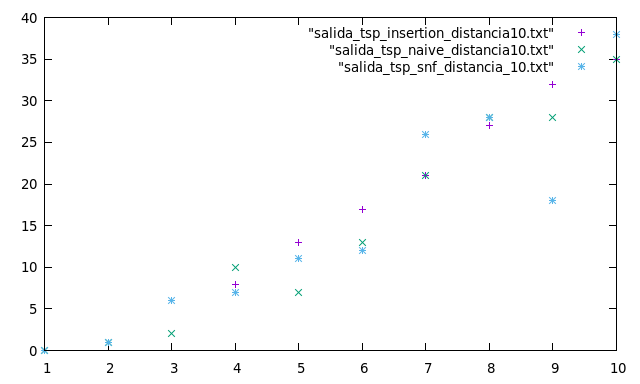
\includegraphics[width=15cm]{../Graficas/graficastsp/distancia3.png}
	\end{center}	
\end{datos}
Podemos ver que las distancias de los tres algoritmos son similares, pero el tiempo que se emplea en obtenerlas es mucho mayor en fuerza bruta. Estudiaremos por tanto los algoritmos \emph{inserción} y \emph{cercanía} por separado. 

\begin{datos}
	{\bf\sffamily Gráfico 1.4.3.} {\sffamily Contraste de datos empíricos (cercanía e inserción): tiempo}\\
	\vspace{-0.7cm}
	\begin{center}
		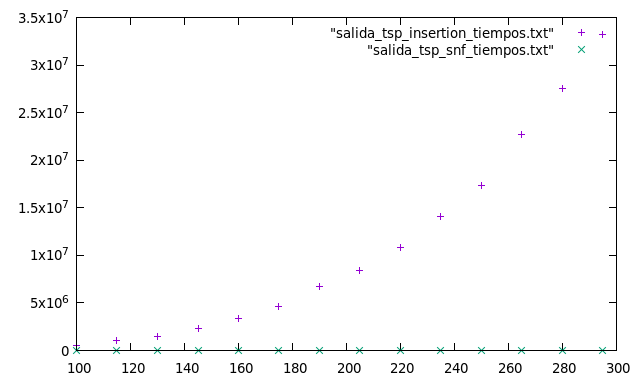
\includegraphics[width=15cm]{../Graficas/graficastsp/tiempo2.png}
	\end{center}	
\end{datos}
\pagebreak
\begin{datos}
	{\bf\sffamily Gráfico 1.4.4.} {\sffamily Contraste de datos empíricos (cercanía e inserción): distancia}\\
	\vspace{-0.7cm}
	\begin{center}
		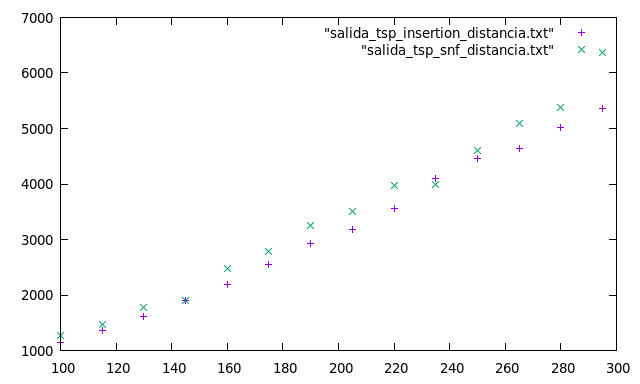
\includegraphics[width=15cm]{../Graficas/graficastsp/distancia2.png}
	\end{center}	
\end{datos}

Observamos que las distancias obtenidas con \emph{inserción} son ligeramente mejores, pero al comparar los tiempos \emph{cercanía} es considerablemente más rápido. Por lo general nos interesará más usar este algoritmo, ya que conseguimos resultados parecidos en un tiempo mucho menor. 

Vamos a comparar ahora el algoritmo \emph{cercanía} con nuestro algoritmo: \emph{perturbaciones}

\begin{datos}
	{\bf\sffamily Gráfico 1.4.5.} {\sffamily Contraste de datos empíricos (cercanía y perturbaciones): tiempo}\\
	\vspace{-0.7cm}
	\begin{center}
		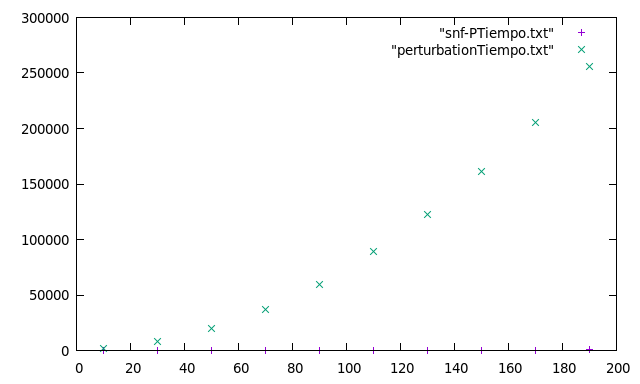
\includegraphics[width=15cm]{../Graficas/graficastsp/TiempoC-P.png}
	\end{center}	
\end{datos}
\begin{datos}
	{\bf\sffamily Gráfico 1.4.6.} {\sffamily Contraste de datos empíricos (cercanía y perturbaciones): distancia}\\
	\vspace{-0.7cm}
	\begin{center}
		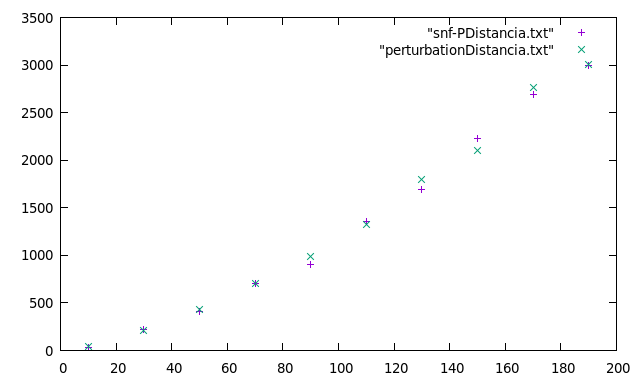
\includegraphics[width=15cm]{../Graficas/graficastsp/DistanciaC-P.png}
	\end{center}	
\end{datos}

Observar que la diferencia de tiempo de nuestro algoritmo es considerable respecto a la de \emph{cercanía} y sin embargo la distancia obtenida es similar. Podemos afirmar por tanto que el algoritmo \emph{cercanía} es mejor que el nuestro. 

\pagebreak

\section{Asignación de tareas (\emph{worker})}

\begin{datos}
	{\sffamily Supongamos que disponemos de \emph{n} trabajadores y \emph{n} tareas. Sea $\text{\sffamily \emph{c}}_\text{\sffamily \emph{ij}} > \text{\sffamily 0}$ el coste de asignarle la tarea \emph{j} al trabajador \emph{i}. Una asignación válida es aquella en la que a cada trabajador le corresponde una tarea y cada tarea la realiza un trabajador diferente. Dada una asignación válida, definimos el coste de dicha asignación como la suma total de los costes individuales. Diseñe un algoritmo voraz para obtener una asignación de tareas a trabajadores óptima.}
\end{datos}

\subsection*{Elementos comunes}

A lo largo de la solución del problema usaremos la siguiente notación:

\begin{itemize}
	\item $n$ es el \textbf{número de trabajadores}, que coincide con el \textbf{número de tareas}.
	\item $C$ es la \textbf{matriz de costes}, de tamaño $n\times n$, en el que el elemento $c_{ij}$ de la matriz es el coste de asignar al trabajador $i$ la tarea $j$.
	\item $a$ es el \textbf{vector de asignaciones}, de tamaño $n$. El trabajo asignado al trabajador $i$ estará contenido en el elemento $a_i$ del vector.
	\item $W_a$ es el coste de una cierta asignación $a$. Se calcula mediante:
	$$ W_a = \sum_{i=0}^{n-1} c_{i,a_i}$$
\end{itemize}

\subsection{Enfoque greedy simple (por inserción)}

Para distribuir las tareas, relizaremos los siguientes pasos:
\begin{enumerate}
	\item Recorremos la matriz $C$ por filas, y asignamos al primer trabajador la tarea de menor coste.
	\item Inhabilitamos la columna haciendo uso de un vector auxiliar $-$que hemos llamado $d$$-$ de trabajos disponibles. También podríamos sobreescribir la matriz $C$ colocando todos los componentes de esa misma columna a 0 $-$pues los costes son siempre estrictamente positivos$-$.
	\item Realizamos de nuevo este procedimiento hasta que todos los trabajadores tengan una tarea asignada, con la salvedad de que en el paso (2) hemos de comprobar si la tarea está disponible $-$comprobando el vector de trabajos disponibles o si los elementos no son ceros, en caso de usar la otra alternativa$-$.
\end{enumerate}

\pagebreak

\begin{table}[h]
\centering
\begin{tabular}{clclclc}
\vspace{0.3cm}(1)&\hspace*{0.8cm}&(2)&\hspace*{0.8cm}&&(3)\\
$C = \left(\begin{matrix}\textbf{2}&4&3\\1&4&2\\2&7&5\\\end{matrix}\right)\begin{matrix}\leftarrow\\\\\\\end{matrix}$&&$C = \left(\begin{matrix}\textcolor{red}{2}&4&3\\\textcolor{red}{1}&4&2\\\textcolor{red}{2}&7&5\\\end{matrix}\right)\begin{matrix}\leftarrow\\\\\\\end{matrix}$&&$C = \left(\begin{matrix}\textcolor{red}{2}&4&3\\\textcolor{red}{1}&4&\textbf{2}\\\textcolor{red}{2}&7&5\\\end{matrix}\right)\begin{matrix}\\\leftarrow\\\\\end{matrix}$&&$C = \left(\begin{matrix}\textcolor{red}{2}&4&\textcolor{red}{3}\\\textcolor{red}{1}&4&\textcolor{red}{2}\\\textcolor{red}{2}&7&\textcolor{red}{5}\\\end{matrix}\right)\begin{matrix}\\\leftarrow\\\\\end{matrix}$\\
$a=\{0,\;,\;\}$&&$a=\{0,\;,\;\}$ &&$a=\{0,2,\;\}$ && $a=\{0,2,\;\}$\\
$d=\{\text{T},\text{T},\text{T}\}$&&$d=\{\text{\textcolor{red}{F}},\text{T},\text{T}\}$&&$d=\{\text{\textcolor{red}{F}},\text{T},\text{T}\}$&&$d=\{\text{\textcolor{red}{F}},\text{T},\text{\textcolor{red}{F}}\}$\\
\end{tabular}
\end{table}

\begin{center}
	\footnotesize{Visualización de los pasos anteriormente descritos}
\end{center}
\vspace{0.3cm}
Este enfoque se traduce en un código que comprende las siguientes funciones:

\begin{itemize}
	\item \texttt{get\_best\_solution}, una función para calcular la asignación especificada anteriormente.
	\item \texttt{find\_best\_task}, una función auxiliar para calcular la mejor tarea que se encuentre disponible (haciendo uso de un vector de disponibles, \texttt{available}), de un conjunto de tareas
\end{itemize}

El código completo se encuentra en la \textbf{\emph{sección IV: Anexo I}} de este documento.

Veremos la eficiencia empírica de este algoritmo.

\subsubsection*{Análisis empírico}
Los tamaños de prueba para ejecutar el algoritmo han ido desde 100 hasta 4000, cada vez con incremento de 200. A su vez cada iteración la hemos hecho 100 veces y hemos calculado la media, con el fin de eliminar los mejores y peores casos.  

Los datos obtenidos, calculando por un lado el tiempo y por otro la distancia han sido estos:
\pagebreak
\begin{datos}
	{\bf\sffamily Gráfico 2.1.1.} {\sffamily Datos empíricos para asignación de tareas, inserción: tiempo}\\
	\vspace{-0.7cm}
	\begin{center}
		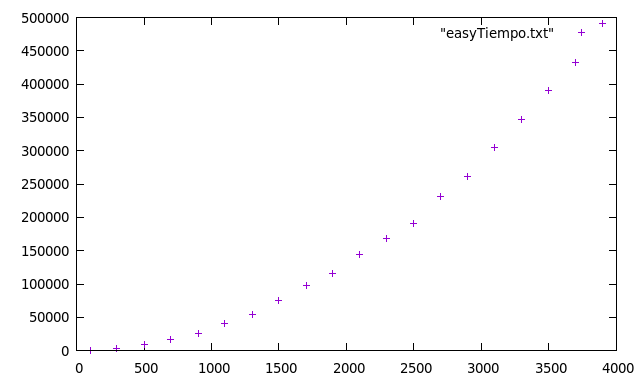
\includegraphics[width=15cm]{../Graficas/graficasWorker/easyTiempo.png}
	\end{center}	
\end{datos}
\begin{datos}
	{\bf\sffamily Gráfico 2.1.2.} {\sffamily Datos empíricos para asignación de tareas, inserción: coste}\\
	\vspace{-0.7cm}
	\begin{center}
	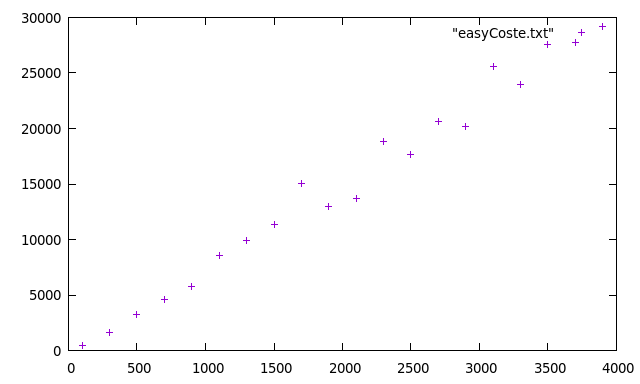
\includegraphics[width=15cm]{../Graficas/graficasWorker/easyCoste.png}
	\end{center}	
\end{datos}

Los datos de las gráficas se encuentran en la \textbf{\emph{sección IV: Anexo II}} de este documento.

\subsection{Enfoque greedy con permutaciones}

Este algoritmo consiste en, partiendo de una asignación, ir modificándola hasta encontrar una mejor, es decir, con una \textbf{ganancia} positiva.

El procedimiento es sencillo:

\begin{enumerate}
	\item Buscamos el elemento que tiene un coste mayor de todas las asignaciones, al que llamaremos $a_m$, con $m$ la posición de dicho elemento.
	\item Vamos intercambiando los elementos del vector de asignaciones con el de coste mayor, es decir, obtenemos las asignaciones resultantes de realizar esta permutación: $$a'_0=\{a_m, a_1, ..., a_{m-1}, a_0, a_{m+1}, ..., a_{n-1}\}, a'_1 = \{a_0, a_m, a_2, ..., a_{m-1}, a_1, a_{m+1}, a_{n-1}\}, ...$$De entre todas las posibilidades, tomaremos la que tiene mayor ganancia, es decir, el $p$ con el $W_{a'_p}$ menor, la que nos proporciona una asignación con menor coste.
	\item Repetimos este proceso un número de veces arbitrario, en cada iteración obtendremos una solución mejor, o la misma solución (en cuyo caso no podremos mejorar esta asignación realizando permutaciones).
\end{enumerate}

Podríamos partir de la asignación que proporciona el enfoque anterior, mejorándola con estas permutaciones.

Este enfoque se traduce en un código que comprende las siguientes funciones:

\begin{itemize}
	\item \texttt{get\_best\_solution}, de nuevo nuestra función principal para resolver el problema.
	\item \texttt{find\_worst\_worker}, una función auxiliar para encontrar el trabajador que tiene la \emph{peor tarea asignada}, es decir, el que tiene mayor costo. Esto se traduce en nuestra implementación a simplemente buscar el máximo del vector $a$, de asignaciones (1).
	\item \texttt{find\_best\_permutation}, una función auxiliar que, de entre todas las permutaciones posibles, encuentra la que tiene una ganancia mayor (2).
	\item \texttt{permutate}, una función auxiliar que efectúa la permutación, es decir, modifica el vector $a$ de asignaciones para efectuar el intercambio encontrado.
\end{itemize}

El código completo se encuentra en la \textbf{\emph{sección IV: Anexo I}} de este documento. En dicho código se parte de las funciones del enfoque anterior: \texttt{get\_best\_solution} (que ha sido renombrado a \texttt{get\_insertion\_solution}) y \texttt{find\_best\_task}.

Veremos la eficiencia empírica de este algoritmo.

\subsubsection*{Análisis empírico}
Los tamaños de prueba para ejecutar el algoritmo han ido desde 1 hasta 100, cada vez con incremento de 10. A su vez cada iteración la hemos hecho 100 veces y hemos calculado la media, con el fin de eliminar los mejores y peores casos.  

Los datos obtenidos, calculando por un lado el tiempo y por otro la distancia han sido estos:

\begin{datos}
	{\bf\sffamily Gráfico 2.2.1.} {\sffamily Datos empíricos para asignación de tareas, perturbaciones: tiempo}\\
	\vspace{-0.7cm}
	\begin{center}
		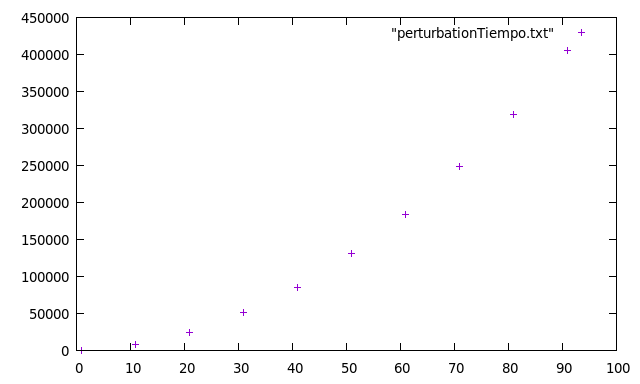
\includegraphics[width=15cm]{../Graficas/graficasWorker/perturbationTiempo.png}
	\end{center}	
\end{datos}

\begin{datos}
	{\bf\sffamily Gráfico 2.2.2.} {\sffamily Datos empíricos para asignación de tareas, perturbaciones: coste}\\
	\vspace{-0.7cm}
	\begin{center}
		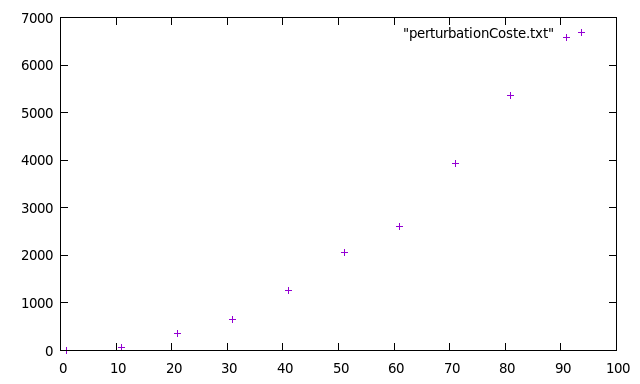
\includegraphics[width=15cm]{../Graficas/graficasWorker/perturbationCoste.png}
	\end{center}	
\end{datos}

Los datos de las gráficas se encuentran en la \textbf{\emph{sección IV: Anexo II}} de este documento.

\subsection{Comparación de enfoques}

Ambos enfoques son \emph{greedy}, e intentan acercarse a la mejor solución. Evidentemente, el primero de ellos, por inserción, no se acerca a la mejor solución de todas. Basta tomar como ejemplo la siguiente matriz de costes:

$$C=\left(\begin{matrix}1&2\\2&10\end{matrix}\right)$$

Éste efectuaría una asignación que tendría un coste de 11, mientras que la asignación óptima para este caso tendría un coste de 4.

Para poder resolver esto, el enfoque con permutaciones es una solución muy interesante. Éste solucionaría nuestro problema en este caso, llegando a la asignación óptima tras una sola permutación.

Además, el enfoque con permutaciones es especialmente interesante cuando partimos de una cantidad muy grande de datos, ya que tener una estimación inicial puede ser complicado. Podríamos partir de una asignación cualquiera, y aplicar estas permutaciones de forma sucesiva hasta encontrar asignaciones mejores con cada iteración. En resumen, podemos dejar a nuestro algoritmo calcular asignaciones consecutivamente mejores, simplemente con dejar un tiempo de ejecución mayor.

Vemos por tanto cómo podemos, a partir de \emph{greedy}, obtener algoritmos que nos \textbf{mejoran} nuestras soluciones conforme van actuando de forma sucesiva.

\subsubsection*{Comparación en análisis empírico}

Comparamos empíricamente los dos algoritmos propuestos y otro hecho por fuerza bruta. Como este último solo funciona para tamaños muy pequeños situamos la cota en 10.

\pagebreak

\begin{datos}
	{\bf\sffamily Gráfico 2.3.1.} {\sffamily Contraste de datos empíricos: tiempo}\\
	\vspace{-0.7cm}
	\begin{center}
		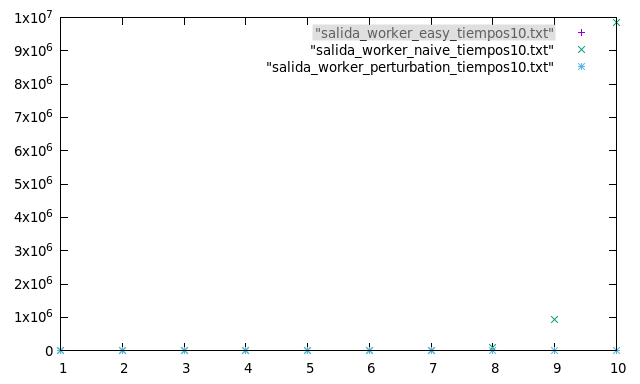
\includegraphics[width=15cm]{../Graficas/graficasWorker/tiempos3.png}
	\end{center}	
\end{datos}

\begin{datos}
	{\bf\sffamily Gráfico 2.3.2.} {\sffamily Contraste de datos empíricos: coste}\\
	\vspace{-0.7cm}
	\begin{center}
		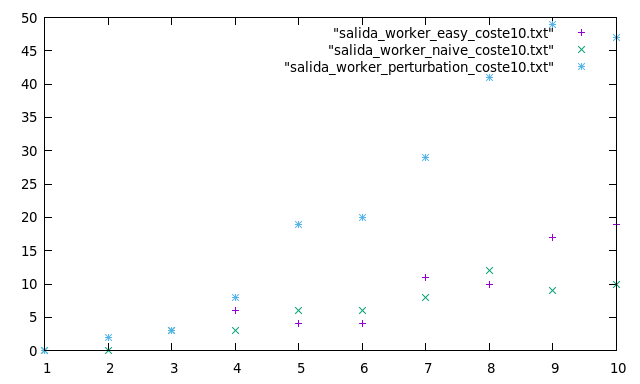
\includegraphics[width=15cm]{../Graficas/graficasWorker/coste3.png}
	\end{center}	
\end{datos}
Vemos que los mayores valores de coste los obtenemos con \emph{perturbations} mientras que con \emph{fuerza bruta} y \emph{easy} se obtienen valores similares. Para el tiempo, sin embargo, los valores de \emph{fuerza bruta} se disparan. Vamos a estudiar por tanto a más largo plazo los dos primeros algoritmos. 
\begin{datos}
	{\bf\sffamily Gráfico 2.3.3.} {\sffamily Contraste de datos empíricos: tiempo}\\
	\vspace{-0.7cm}
	\begin{center}
		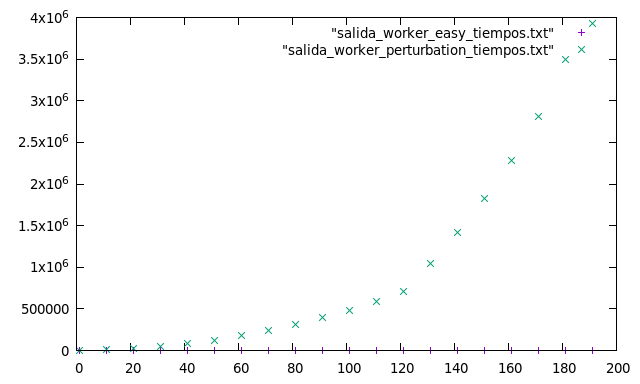
\includegraphics[width=15cm]{../Graficas/graficasWorker/tiempos2.png}
	\end{center}	
\end{datos}
\begin{datos}
	{\bf\sffamily Gráfico 2.3.4.} {\sffamily Contraste de datos empíricos: coste}\\
	\vspace{-0.7cm}
	\begin{center}
		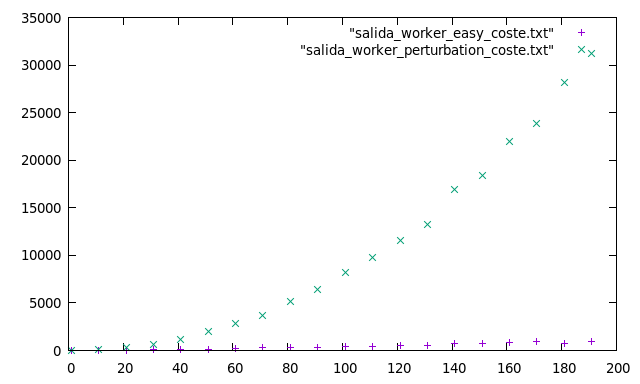
\includegraphics[width=15cm]{../Graficas/graficasWorker/coste2.png}
	\end{center}	
\end{datos}
Observar que la gráfica de \emph{perturbations} crece más rápida tanto en tiempo que podemos decir que el algoritmo \emph{easy} es mejor.

\pagebreak
\part{Conclusiones}

Con esta práctica, hemos aprendido a crear algoritmos voraces para resolver problemas que, en su versión en fuerza bruta, tienen una complejidad muy elevada.

Hemos contemplado, dentro de esta técnica, diversos enfoques para cada algoritmo, prestando atención a la dificultad de obtener la solución óptima, y primando el ``acercarnos'' a ella mediante algoritmos que, con sucesivas iteraciones, van mejorando la solución anterior, hasta llegar a soluciones cada vez más óptimas.

Esto es algo de especial relevancia al trabajar con cantidades ingentes de datos, en el que dar una solución inicial puede ser muy complicada, pudiendo partir incluso de soluciones arbitrarias, mejorándolas conforme nuestros algoritmos se van ejecutando.

\pagebreak

\part{Anexos}

\section*{Anexo I. Códigos}

\subsection*{Códigos para TSP}

\subsubsection*{\texttt{tsp\_common.hpp}}

Biblioteca de \textbf{funciones comunes} a todos los códigos usados.

\begin{lstlisting}[language=C]
#include <vector>
#include <stdlib.h>
#include <time.h>
#include <cstdlib>

namespace common{

// Generacion de numeros aleatorios
//==============================================================================

/**
 * @brief Devuelve el valor absoluto de un valor double 
 * @param val el double con el que trabajamos
 * @return el valor absoluto de un valor double
 * */
double abs(double val){
    return val < 0 ? - val : val;
}

void startRandom(){
    std::srand(time(NULL));
}

int randomInt(int min, int max){
    int value = min + std::rand() % (max +1 - min) ;
    return value;
} 

double random_double(double min, double max){
    return (std::rand() / (double) RAND_MAX ) * (max - min) + min;
}

// Estructura basicas Punto
//==============================================================================
/**
 * @brief Estructura para representar un punto en el plano
 *
 * En esta estructura se implementa la distancia base que usa el resto de las funciones
 * */
struct Point{
    double x = 0;
    double y = 0;

    /**
     * @brief Distancia entre dos puntos
     *
     * Cambiar esta funcion si queremos cambiar la distancia entre dos puntos para 
     * cualquier funcion que haga uso de la distancia (esta es la implementacion base)
     * */
    double distance(Point other){
        return abs(other.x - x) + abs(other.y - y);
    }
};

// Generacion de datos para el problema
//==============================================================================

/**
 * @brief Genera los puntos necesarios para el problema
 * @param num_points, la cantidad de puntos con la que queremos trabajar
 * @return un vector de puntos, cuyas coordenadas estan en el intevalo [0, num_points]
 * */
std::vector<Point> generate_problem_data(int num_points){
    std::vector<Point> points;

    for(int i = 0; i < num_points; i++){
        double x = random_double(0, num_points);
        double y = random_double(0, num_points);

        Point p = {x, y};
        points.push_back(p);
    }

    return points;
}

// Funcionalidades para solucionar partes comunes del problema
//==============================================================================

/**
 * @brief Genera un camino dado una permutacion de indices
 * @param points, los puntos sobre los que queremos calcular el camino
 * @param permutation, la permutacion de indices
 * @return un camino dado los puntos y la permutacion
 * */
std::vector<Point> generate_road_by_indexes(std::vector<common::Point> points, std::vector<int> permutation){
    std::vector<Point> road;

    for(auto index : permutation){
        road.push_back(points[index]);
    }

    return road;
}

/**
 * @brief Genera el camino resultado de intercambiar dos posiciones de un camino
 * @param road, el camino base
 * @param pos1, la primera posicon con la que intercambiamos
 * @param pos2, la segunda posicon con la que intercambiamos
 * @return un camino resultado del cambio descrito
 * */
std::vector<Point> get_swap(std::vector<Point> road, int pos1, int pos2){
    std::vector<Point> changed = road;

    Point tmp = road[pos1];
    road[pos1] = road[pos2];
    road[pos2] = tmp;

    return changed;
}

// Calculo de distancias
//==============================================================================
/**
 * @brief Calcula la distancia entre dos puntos
 * @param p1, el primer punto del que queremos calcular la distancia
 * @param p2, el segundo punto del que queremos calcular la distancia
 * @return al distancia entre ambos puntos
 * */
double distance(Point p1, Point p2){
    return p1.distance(p2);
}

/**
 * @brief Calcula la distancia de un camino dado
 * @param road, vector de puntos que forman un camino
 * @return la distancia total de ese camino
 * */
double get_road_distance(std::vector<Point> road){
    double road_distance = 0;

    // Distancia entre los n puntos
    for(int i = 0; i < road.size() - 1; i++){
        road_distance = road_distance + distance(road[i], road[i+1]);

    }

    // Distancia entre el ultimo y primer punto
    road_distance = road_distance + distance(road[0], road[road.size()-1]);

    return road_distance;
}

} // namespace common
\end{lstlisting}

\subsubsection*{\texttt{tsp\_naive.cpp}}

Resolución del algoritmo por \textbf{fuerza bruta}.

\begin{lstlisting}[language=C]
#include <vector>
#include <string>
#include <iostream>
#include <algorithm>
#include "tsp_common.hpp"
using namespace std;

// Declaracion de las funciones que vamos a calcular
//==============================================================================

/**
 * @brief Genera todas las permutaciones posibles del conjunto {0, 1, ..., n-1}
 * @return un vector con todas las permutaciones posibles
 * */
vector<vector<int> > generate_permutations(int n);

/**
 * @brief Calcula la mejor solucion para un conjunto de puntos, por fuerza bruta
 * @param points, el conjunto de puntos sobre el que vamos a operar
 * @return el camino cuya distancia es la minima
 * */
vector<common::Point> get_best_solution(vector<common::Point> points);



int main(){
    // Parametro del programa para probar cosas
    int num_points = 10;

    // Puntos con los que voy a trabajar
    vector<common::Point> points = common::generate_problem_data(10);

    // Soluciono el problema por fuerza bruta
    vector<common::Point> road = get_best_solution(points);

    // Muestro el resultado del problema
    cout << "El camino optimo para el problemma es: " << endl;
    for(auto point : road){
        cout << "x: " << point.x << " y: " << point.y << endl;
    }

    cout << "La distancia del camino optimo es: " << get_road_distance(road) << endl;


    // Todo ha salido OK
    return 0;
}

// Implementacion de las funciones
//==============================================================================
vector<vector<int> > generate_permutations(int n){
    vector<vector<int> > permutations;

    // We get the base permutation to work with
    vector<int> base_perm;
    for(int i = 0; i < n; i++){
        base_perm.push_back(i);
    }

    do{
        permutations.push_back(base_perm);
    }while(next_permutation(base_perm.begin(), base_perm.end()));


    return permutations;
}

vector<common::Point> get_best_solution(vector<common::Point> points){
    // Permutaciones con las que vamos a trabajar
    vector<vector<int> > permutations = generate_permutations(points.size());

    // Camino y distancia minima
    vector<common::Point> min_road = points;
    double min_distance = common::get_road_distance(min_road);

    // Calculo las distancias de todas las permutaciones
    for(auto permutation : permutations){
        vector<common::Point> current_road = common::generate_road_by_indexes(points, permutation);
        double current_distance = common::get_road_distance(current_road);

        if(current_distance < min_distance){
            min_distance = current_distance;
            min_road = current_road;
        }
    }

    return min_road;
}
\end{lstlisting}

\subsubsection*{\texttt{tsp\_matrix.cpp}}

Resolución usando \textbf{matrices de distancias}.

\begin{lstlisting}[language=C]
#include <iostream>
#include <vector>
#include "tsp_common.hpp"
using namespace std;

// Declaracion de funciones con las que trabajamos
//==============================================================================

/**
 * @brief Calcula la mejor solucion para un conjunto de puntos, por Shortest Neighbor First
 * @param points, el conjunto de puntos sobre el que vamos a operar
 * @pre points.size() > 0
 * @return el camino cuya distancia es la minima, si todo sale bien
 *         un vector vacio, si ocurre algun error
 * */
vector<common::Point> get_best_solution(vector<common::Point> points);

/**
 * @brief Genera una matriz con las distancias entre los puntos 
 * @param points, los puntos sobre los que calculamos las distancias
 * @return una matriz con las distancias entre los puntos
 *
 * Matriz[i][j] := distance(pi, pj)
 *
 *
 * WIP -- Tiene una violacion del segmento
 * */
vector<vector<double> > generate_distances_matrix(vector<common::Point> points);

/**
 * @brief Limpia las distancias de una determinada posicion
 *        Ello implica poner a cero la fila y columna de una determinada posicion
 * @param distances_matrix, matriz sobre la que trabajamos, SE MODIFICA
 * @param pos, la posicion sobre la que tenemos que limpiar
 * */
void clean_position(vector<vector<double> > & distances_matrix, int pos);

/**
 * @brief Halla la posicion en una fila con la menor distancia
 * @param distances_matrix, la matriz con las distancias
 * @param position, la posicion respecto la que queremos buscar el minimo elemento
 * @return la posicion cuya distancia es la minima, si todo sale bien
 *         -1, si ocurre algun error
 * */
int get_min_row_element(vector<vector<double> > distances_matrix, int position);

/**
 * @brief Genera una matriz size x size llena de ceros
 * @parma size, la dimension de la matriz cuadrada
 * @return la matriz cuadrada llena de ceros
 * */
vector<vector<double> > get_empty_matrix(int size);

// Funcion principal
//==============================================================================
int main(){
    // Parametro sobre el size del problema
    int problem_size = 100;

    // Inicio los numeros aleatorios
    common::startRandom();

    // Puntos con los que vamos a trabajar
    vector<common::Point> points = common::generate_problem_data(problem_size);

    // Calculo la solucion aproximada
    vector<common::Point> road = get_best_solution(points);

    // Muestro el resultado
    cout << "La distancia de la solucion obtenida es: " << common::get_road_distance(road) << endl;

    // Todo ha salido OK
    return 0;
}

// Implementacion de las funciones 
//==============================================================================
void clean_position(vector<vector<double> > & distances_matrix, int pos){
    // Cleaning the row
    for(int col = 0; col < distances_matrix.size(); col++){
        distances_matrix[pos][col] = 0;
    }

    // Cleaning the col
    for(int row = 0; row < distances_matrix.size(); row++){
        distances_matrix[row][pos] = 0;
    }
}

int get_min_row_element(vector<vector<double> > distances_matrix, int position){
    int min_pos = 0;
    int starting_pos = 0;

    // Busco la primera posicion con distancia no nula
    while(distances_matrix[position][starting_pos] == 0 && starting_pos < distances_matrix.size()){
        starting_pos = starting_pos + 1;
    }

    // Comprobacion de seguridad
    if(starting_pos = distances_matrix.size()-1){
        cerr << "ERROR! Posicion no encontrada en get_min_row_element()" << endl;
        cerr << "Se devuelve -1 como codigo de error!" << endl;
        return -1;
    }

    // Busco el elemento optimo de la columna
    min_pos = starting_pos;
    double min_val = distances_matrix[position][starting_pos];

    for(int col = starting_pos; col < distances_matrix[position].size(); col++){
        if(distances_matrix[position][col] < min_val){
            min_pos = col;
            min_val = distances_matrix[position][col];
        }
    }

    return min_pos;
}

vector<common::Point> get_best_solution(vector<common::Point> points){
    vector<common::Point> road;
    vector<vector<double> > distances_matrix = generate_distances_matrix(points);

    // WIP
    for(int row = 0; row < distances_matrix.size(); row++){
        for(int col = 0; col < distances_matrix.size(); col++){
            cout << distances_matrix[row][col] << " ";
        }
        cout << endl;
    }
 
    // Empiezo siempre por el primer punto
    int last_point = 0;
    road.push_back(points[0]);

    while(road.size() < points.size()){
        // Hallo el punto mas cercano al anterior
        int best_position = get_min_row_element(distances_matrix, last_point);

        // Comprobacion de seguridad
        if(best_position == -1){
            cerr << "ERROR! Posicion optima no encontrada en get_best_solution()" << endl;
            cerr << "Se devuelve un vector nulo!" << endl;

            // Devuelvo un vector vacio
            return vector<common::Point>();
        }

        // Lo inserto al road
        road.push_back(points[best_position]);
        
        // Limpio la fila y columna del anterior punto, ya no me hace falta
        clean_position(distances_matrix, best_position);

        // Tomo el nuevo punto anterior
        last_point = best_position;
    }

    return road;
}

vector<vector<double> > generate_distances_matrix(vector<common::Point> points){
    // Genero una matriz de points.size() x points.size() llena de ceros
    vector<vector<double> > distances_matrix = get_empty_matrix(points.size());

    for(int row = 0; row < points.size(); row++){
        for(int col = 0; col < points.size(); col++){
            distances_matrix[row][col] = common::distance(points[row], points[col]);
        }
    }       

    return distances_matrix;
}

vector<vector<double> > get_empty_matrix(int size){
    vector<vector<double> > empty;
    vector<double> empty_row(size, 0);

    for(int i = 0; i < size; i++){
        empty.push_back(empty_row);
    }

    return empty;
}
\end{lstlisting}

\subsubsection*{\texttt{tsp\_snf.cpp}}

Solución por \textbf{SNF} usando un vector con los puntos que quedan.

\begin{lstlisting}[language=C]
#include <iostream>
#include <vector>
#include "tsp_common.hpp"
using namespace std;

// Declaracion de funciones con las que trabajamos
//==============================================================================

/**
 * @brief Calcula la mejor solucion para un conjunto de puntos, por Shortest Neighbor First
 * @param points, el conjunto de puntos sobre el que vamos a operar
 * @pre points.size() > 0
 * @return el camino cuya distancia es la minima
 * */
vector<common::Point> get_best_solution(vector<common::Point> points);

// Funcion principal
//==============================================================================
int main(){
    // Parametro sobre el size del problema
    int problem_size = 10000;

    // Inicio los numeros aleatorios
    common::startRandom();

    // Puntos con los que vamos a trabajar
    vector<common::Point> points = common::generate_problem_data(problem_size);

    // Calculo la solucion aproximada
    vector<common::Point> road = get_best_solution(points);

    // Muestro el resultado
    cout << "La distancia de la solucion obtenida es: " << common::get_road_distance(road) << endl;

    // Todo ha salido OK
    return 0;
}

// Implementacion de las funciones 
//==============================================================================
vector<common::Point> get_best_solution(vector<common::Point> points){
    vector<common::Point> road;                 // Solucion que vamos a construir
    vector<common::Point> points_left = points; // Puntos que quedan por insertar a la solucion

    // Parto siempre del primer punto del vector
    road.push_back(points_left[0]);
    points_left.erase(points_left.begin() + 0);

    // Voy construyendo la solucion, sacando puntos de points_left y colocandolos en road
    while(points_left.size() > 0){
        double min_distance = common::distance(road[road.size() -1], points_left[0]);
        int min_pos = 0;

        // Buscamos el punto mas cercano
        for(int i = 0; i < points_left.size(); i++){
            double current_distance = common::distance(road[road.size() -1], points_left[i]);
            if(current_distance < min_distance){
                min_distance = current_distance;
                min_pos = i;
            }
        }

        // Insertamos el punto mas cercano a la solucion y lo quitamos de los puntos que faltan
        road.push_back(points_left[min_pos]);
        points_left.erase(points_left.begin() + min_pos);
    }

    return road;
}
\end{lstlisting}

\subsubsection*{\texttt{tsp\_perturbation.cpp}}

Solución usando \textbf{perturbaciones}, partiendo del SNF anterior.

\begin{lstlisting}[language=C]
#include <iostream>
#include <vector>
#include "tsp_common.hpp"
using namespace std;

// Declaracion de funciones con las que trabajamos
//==============================================================================

/**
 * @brief Calcula la solucion para un conjunto de puntos, por Shortest Neighbor First
 * @param points, el conjunto de puntos sobre el que vamos a operar
 * @pre points.size() > 0
 * @return el camino siguiendo este algoritmo
 * */
vector<common::Point> get_snf_solution(vector<common::Point> points);

/**
 * @brief Calcula un camino partiendo de un algoritmo SNF y aplicandole una serie de perturbaciones
 * @param points, conjunto de puntos sobre el que calcular el mejor camino posible
 * @parma perturbations, numero de perturbaciones que se van a realizar
 * @return el camino obtenido como ya se ha descrito
 * */
vector<common::Point> get_best_solution(vector<common::Point> points, int perturbations);

/**
 * @brief Perturba un camino respecto de un punto dado
 * @brief road, el camino a perturbar, SE MODIFICA
 * @param pos, la posicion respecto la que se perturba
 * */
void perturbate(vector<common::Point> road, int pos);

/**
 * @brief Calcula el punto cuya distancia al siguiente punto es mayor
 * @param road, camino cuyo peor camino hay que calcular 
 * @return la posicion del peor punto ya descrito
 * */
int get_worst_node(vector<common::Point> road);

// Funcion principal
//==============================================================================
int main(){
    // Parametro sobre el size del problema
    int problem_size = 100;
    int perturbations = 100;

    // Inicio los numeros aleatorios
    common::startRandom();

    // Puntos con los que vamos a trabajar
    vector<common::Point> points = common::generate_problem_data(problem_size);

    // Calculo la solucion aproximada
    vector<common::Point> road = get_best_solution(points, perturbations);

    // Muestro el resultado
    cout << "La distancia de la solucion obtenida es: " << common::get_road_distance(road) << endl;

    // Todo ha salido OK
    return 0;
}

// Implementacion de las funciones 
//==============================================================================
vector<common::Point> get_snf_solution(vector<common::Point> points){
    vector<common::Point> road;                 // Solucion que vamos a construir
    vector<common::Point> points_left = points; // Puntos que quedan por insertar a la solucion

    // Parto siempre del primer punto del vector
    road.push_back(points_left[0]);
    points_left.erase(points_left.begin() + 0);

    // Voy construyendo la solucion, sacando puntos de points_left y colocandolos en road
    while(points_left.size() > 0){
        double min_distance = common::distance(road[road.size() -1], points_left[0]);
        int min_pos = 0;

        // Buscamos el punto mas cercano
        for(int i = 0; i < points_left.size(); i++){
            double current_distance = common::distance(road[road.size() -1], points_left[i]);
            if(current_distance < min_distance){
                min_distance = current_distance;
                min_pos = i;
            }
        }

        // Insertamos el punto mas cercano a la solucion y lo quitamos de los puntos que faltan
        road.push_back(points_left[min_pos]);
        points_left.erase(points_left.begin() + min_pos);
    }

    return road;
}

vector<common::Point> get_best_solution(vector<common::Point> points, int perturbations){
    // Tomo la solucion dada por el snf
    vector<common::Point> base_road = get_snf_solution(points);

    // Perturbo el numero de veces indicada
    for(int i = 0; i < perturbations; i++){
        // Calculo la posicion respecto a la que perturbar
        int pos = get_worst_node(points);

        // Perturbo el camino base
        perturbate(base_road, pos);
    }

    return base_road;
}

void perturbate(vector<common::Point> road, int pos){
    vector<common::Point> current_perb = road;
    double best_gain = 0;
    int best_perturbation = pos;
    double base_distance = common::get_road_distance(road);
    
    // Calculo la distancia de todas las permutaciones
    for(int i = 0; i < road.size(); i++){
        // Calculo la ganancia de esta permutacion
        current_perb = common::get_swap(road, pos, i);
        double swap_distance = common::get_road_distance(current_perb);
        double current_gain = swap_distance - base_distance;

        // Compruebo si he mejorado la ganancia
        if(current_gain > best_gain){
            best_perturbation = i;
            best_gain = current_gain;
        }
    }

    // Hago el cambio con la mejor perturbacion
    road = common::get_swap(road, pos, best_perturbation);
}

int get_worst_node(vector<common::Point> road){
    double worst_distance = common::distance(road[0], road[1]);
    int worst_pos = 0;

    // Recorro todos los puntos para ver cual es el peor
    for(int i = 0; i < road.size() - 1; i++){
        if(distance(road[i], road[i+1]) > worst_distance){
            worst_distance = distance(road[i], road[i+1]);
            worst_pos = i;
        }
    }

    // Compruebo la distancia del ultimo al primero
    if(distance(road[road.size()-1], road[0]) > worst_distance){
        worst_distance = road.size() - 1;
    }

    return worst_pos;
}
\end{lstlisting}

\subsection*{Códigos para \emph{worker}}

\subsubsection*{\texttt{worker\_common.cpp}}

Biblioteca de \textbf{funciones comunes} a todos los códigos usados.

\begin{lstlisting}[language=C]
#include <iostream>
#include <vector>
#include <stdlib.h>
#include <time.h>
#include <cstdlib>

namespace common{

// Generacion de numeros aleatorios
//==============================================================================

/**
 * @brief Devuelve el valor absoluto de un valor double 
 * @param val el double con el que trabajamos
 * @return el valor absoluto de un valor double
 * */
double abs(double val){
    return val < 0 ? - val : val;
}

/**
 * @brief inicia la generacion de numeros aleatorios
 * */
void startRandom(){
    std::srand(time(NULL));
}

/**
 * @brief Genera un double aleatorio en un intervalo dado
 * @param min, el minimo valor que se puede tomar
 * @param max, el maximo valor que se puede tomar
 * @return un double en el intervalo [min, max]
 * */
double random_double(double min, double max){
    return (std::rand() / (double) RAND_MAX ) * (max - min) + min;
}

/**
 * @brief Genera un entero aleatorio en un intervalo dado
 * @param min, el minimo valor que se puede tomar
 * @param max, el maximo valor que se puede tomar
 * @return un entero en el intervalo [min, max]
 * */
double random_int(int min, int max){
    return (int)(std::rand() / (double) RAND_MAX ) * (max - min) + min;
}

// Generacion de los datos del problema
//==============================================================================
/**
 * @brief Genera una matriz aleatoria con las asignaciones de trabajo
 * @param size, size del problema (no. de trabajadores y trabajos)
 * @return una matriz cuadrada de dimension size con valores aleatorios en el intervalo [0, size]
 * */
std::vector<std::vector<double> > generate_matrix(int size){
    // Inicio una matriz llena de ceros
    std::vector<double> empty_row(size, 0);
    std::vector<std::vector<double> > matrix(size, empty_row);

    for(int row = 0; row < size; row++){
        for(int col = 0; col < size; col++){
            matrix[row][col] = random_double(0, size);
        }
    }

    return matrix;
}

// Calculos sobre datos del problema
//==============================================================================
/**
 * @brief Calcula el coste de una asignacion dada
 * @param matrix, la matriz con los costes
 * @param asignation, la asignacion cuyo coste se calcula
 * @return el coste de la asignacion
 * */
double get_cost(std::vector<std::vector<double> > matrix, std::vector<int> asignation){
    double cost = 0;

    for(int i = 0; i < asignation.size(); i++){
        cost = cost + matrix[i][asignation[i]];
    }

    return cost;
}

// Muestra de datos del problema
//==============================================================================
void show_matrix(std::vector<std::vector<double> > matrix, char sep = '\t'){
    for(int row = 0; row < matrix.size(); row++){
        for(int col = 0; col < matrix[row].size(); col++){
            std::cout << matrix[row][col] << sep;
        }
        std::cout << std::endl;
    }
}
    
}// namespace common
\end{lstlisting}

\subsubsection*{\texttt{worker\_naive.cpp}}

Resolución mediante \textbf{fuerza bruta}.

\begin{lstlisting}[language=C]
#include <iostream>
#include <vector>
#include <algorithm>
#include "worker_common.hpp"
using namespace std;

// Declaracion de funciones auxiliares
//==============================================================================
/**
 * @brief Genera todas las permutaciones del conjunto {0, 1, ..., n-1}
 * @param n, el maximo del conjunto sobre el que se permuta
 * @return un array con todas las permutaciones anteriormente descritas
 * */
vector<vector<int> > generate_permutations(int n);

/**
 * @brief Calcula la asignacion optima dada una matriz de costes, usando fuerza bruta
 * @param matrix, la matriz que almacena los costes
 * @return la asignacion optima
 * */
vector<int> get_best_solution(vector<vector<double> > matrix);

// Funcion principal
//==============================================================================
int main(){
    // Parametro para hacer pruebas con las entradas
    int size = 4;

    // Inicio la generacion de numeros aleatorios
    common::startRandom();

    // Tomo una matriz con los datos del problema
    vector<vector<double> > worker_matrix = common::generate_matrix(size);

    // Calculo la solucion al problema
    vector<int> asignation = get_best_solution(worker_matrix);

    // Muestro el coste de la solucion optima
    cout << "El coste optimo es: " << common::get_cost(worker_matrix, asignation) << endl;

    // Muestro las asignaciones hechas
    for(int i = 0; i < size; i++){
        cout << "Trabajador " << i << " asignado al trabajo " << asignation[i] << endl;
    }

    // Todo ha salido OK
    return 0;
}

// Implementacion de funciones auxiliares
//==============================================================================
vector<vector<int> > generate_permutations(int n){
    vector<vector<int> > permutations;

    // We get the base permutation to work with
    vector<int> base_perm;
    for(int i = 0; i < n; i++){
        base_perm.push_back(i);
    }

    do{
        permutations.push_back(base_perm);
    }while(next_permutation(base_perm.begin(), base_perm.end()));


    return permutations;
}

vector<int> get_best_solution(vector<vector<double> > matrix){
    // Tomo el array de permutaciones, del que me tengo que quedar con solo una 
    // permutacion, la permutacion de la asignacion optima
    vector<vector<int> > permutations = generate_permutations(matrix.size());

    // Valores base para empezar a realizar comparaciones
    int best_permutation = 0;
    double best_cost = common::get_cost(matrix, permutations[0]);

    // Comparo todas las permutaciones
    for(int i = 0; i < permutations.size(); i++){
        double current_cost = common::get_cost(matrix, permutations[i]);

        if(current_cost < best_cost){
            best_cost = current_cost;
            best_permutation = i;
        }
    }

    return permutations[best_permutation];
}
\end{lstlisting}

\subsubsection*{\texttt{worker\_easy.cpp}}

Resolución del problema haciendo uso de \textbf{greedy}, en el enfoque simple.

\begin{lstlisting}[language=C]
#include <iostream>
#include <vector>
#include <algorithm>
#include "worker_common.hpp"
using namespace std;

// Declaracion de funciones auxiliares
//==============================================================================
/**
 * @brief Calcula la asignacion parcialmente optima dada una matriz de costes, usando un algoritmo greedy
 * @param matrix, la matriz que almacena los costes
 * @return la asignacion parcialmente optima
 * */
vector<int> get_best_solution(vector<vector<double> > matrix);

/**
 * @brief Halla dado un vector de costo de tareas, la mejor tarea que se encuentra disponible
 * @param tasks_cost, vector con los costos de las tareas
 * @param available, vector para controlar si las tareas se encuentra o no disponibles
 * */
int find_best_task(vector<double>tasks_cost, vector<bool> available);

// Funcion principal
//==============================================================================
int main(){
    // Parametro para hacer pruebas con las entradas
    int size = 4000;

    // Inicio la generacion de numeros aleatorios
    common::startRandom();

    // Tomo una matriz con los datos del problema
    vector<vector<double> > worker_matrix = common::generate_matrix(size);

    // Calculo la solucion al problema
    vector<int> asignation = get_best_solution(worker_matrix);

    // Muestro el coste de la solucion optima
    cout << "El coste optimo es: " << common::get_cost(worker_matrix, asignation) << endl;

    // Muestro las asignaciones hechas
    for(int i = 0; i < size; i++){
        cout << "Trabajador " << i << " asignado al trabajo " << asignation[i] << endl;
    }

    // Todo ha salido OK
    return 0;
}

// Implementacion de funciones auxiliares
//==============================================================================
vector<vector<int> > generate_permutations(int n){
    vector<vector<int> > permutations;

    // We get the base permutation to work with
    vector<int> base_perm;
    for(int i = 0; i < n; i++){
        base_perm.push_back(i);
    }

    do{
        permutations.push_back(base_perm);
    }while(next_permutation(base_perm.begin(), base_perm.end()));


    return permutations;
}

vector<int> get_best_solution(vector<vector<double> > matrix){
    // Vector que almacena las tareas que todavia no han sido asignadas
    vector<bool> available_tasks(matrix.size(), true);

    // Vector con la solucion parcial
    vector<int> asignation;

    // Asigno a cada trabajador la tarea con menor coste que quede disponible
    for(int i = 0; i < matrix.size(); i++){
        // Busco la mejor tarea que quede disponible
        int current_task = find_best_task(matrix[i], available_tasks);

        // Insertamos la tarea a la asignacion
        asignation.push_back(current_task);

        // Esa tarea ya no esta disponible
        available_tasks[current_task] = false;
    }

    return asignation;
}

int find_best_task(vector<double>tasks_cost, vector<bool> available){
    // Encuentro la primera tarea disponible para comenzar las comparaciones
    int best_task = 0;
    while(available[best_task] == false){
        best_task++;
    }
    double best_cost = tasks_cost[best_task];

    // Comparo todos los costes que quedan disponibles
    for(int i = best_task; i < tasks_cost.size(); i++){
        if(available[i] == true){ // La tarea sigue disponible
            if(tasks_cost[i] < best_cost){
                best_cost = tasks_cost[i];
                best_task = i;
            }
        }
    }

    return best_task;
}
\end{lstlisting}

\subsubsection*{\texttt{worker\_perturbation.cpp}}

Resolución usando \textbf{perturbaciones}, para ser usado partiendo de una estimación inicial.

\begin{lstlisting}[language=C]
#include <iostream>
#include <vector>
#include <algorithm>
#include "worker_common.hpp"
using namespace std;

// Declaracion de funciones auxiliares
//==============================================================================

/**
 * @brief Calcula la asignacion parcialmente optima dada una matriz de costes, 
 *        usando un algoritmo greedy a partir de una solucion parcial por insercion
 * @param matrix, la matriz que almacena los costes
 * @param num_permutations, el numero de perturbaciones que se van a realizar para mejorar la matriz
 * @return la asignacion parcialmente optima
 * */
vector<int> get_best_solution(vector<vector<double> > matrix, int num_permutations);

/**
 * @brief Encuentra el trabajador con peor coste
 * @param matrix, la matriz con los costes 
 * @param asignation, la asignacion de la que se tiene que encontrar el peor trabajador
 * */
int find_worst_worker(vector<vector<double> > matrix, vector<int> asignation);

/**
 * @brief Encuentra cual es la mejor permutacion para mejorar el coste de una asignacion
 * @param matrix, la matriz con los costes asociados
 * @param base_asignation, asignacion base que tenemos que mejorar
 * @param worst_worker, trabajador con pero coste, el cual se tiene que intercambiar con otro
 * @return el indice del trabajador con el que se tiene que intercambiar el peor trabajador
 * */
int find_best_permutation(vector<vector<double> > matrix, vector<int> base_asignation, int worst_worker);

/**
 * @brief Realiza un intercambio entre trabajadores
 * @param base_asignation, asignacion sobre la que realizamos el intercambio, SE MODIFICA
 * @param first_worker, indice del trabajador que se intercambia
 * @param second_worker, indice del otro trabajador que se intercambia
 * */
void perturbate(vector<int> & base_asignation, int first_worker, int second_worker);

/**
 * @brief Calcula la asignacion parcialmente optima dada una matriz de costes, 
 *        usando un algoritmo greedy
 * @param matrix, la matriz que almacena los costes
 * @return la asignacion parcialmente optima
 * */
vector<int> get_insertion_solution(vector<vector<double> > matrix);

/**
 * @brief Halla dado un vector de costo de tareas, la mejor tarea que se encuentra disponible
 * @param tasks_cost, vector con los costos de las tareas
 * @param available, vector para controlar si las tareas se encuentra o no disponibles
 * */
int find_best_task(vector<double>tasks_cost, vector<bool> available);
        
// Funcion principal
//==============================================================================
int main(){
    // Parametros para hacer pruebas con las entradas
    int size = 400;
    int num_permutations = 20;

    // Inicio la generacion de numeros aleatorios
    common::startRandom();

    // Tomo una matriz con los datos del problema
    vector<vector<double> > worker_matrix = common::generate_matrix(size);

    // Calculo la solucion al problema
    vector<int> asignation = get_best_solution(worker_matrix, num_permutations);

    // Muestro las asignaciones hechas
    for(int i = 0; i < size; i++){
        cout << "Trabajador " << i << " asignado al trabajo " << asignation[i] << endl;
    }

    // Muestro el coste de la solucion optima
    cout << "El coste optimo es: " << common::get_cost(worker_matrix, asignation) << endl;

    // Todo ha salido OK
    return 0;
}

// Implementacion de funciones auxiliares
//==============================================================================
vector<int> get_best_solution(vector<vector<double> > matrix, int num_permutations){
    // Parto de la solucion parcial del greedy por insercion
    vector<int> base_asignation = get_insertion_solution(matrix.size());

    // Hacemos el numero de perturbaciones dado
    for(int i = 0; i < num_permutations; i++){
        // Busco cual es el trabajador con mayor coste
        int worst_worker = find_worst_worker(matrix, base_asignation);
        
        // Busco cual es la mejor permutacion
        int best_permutation = find_best_permutation(matrix, base_asignation, worst_worker);

        // Hago el cambio si hay un cambio a mejor
        perturbate(base_asignation, worst_worker, best_permutation);
    }

    return base_asignation;
}

int find_worst_worker(vector<vector<double> > matrix, vector<int> asignation){
    double worst_cost = matrix[0][asignation[0]];
    int worst_worker = 0;

    for(int i = 0; i < asignation.size(); i++){
        if(matrix[i][asignation[i]] > worst_cost){
            worst_cost = matrix[i][asignation[i]];
            worst_worker = i;
        }
    }

    return worst_worker;
}

int find_best_permutation(vector<vector<double> > matrix, vector<int> base_asignation, int worst_worker){
    // Coste base y coste de cada iteracion
    double base_cost = common::get_cost(matrix, base_asignation);         

    // Genero una perturbacion aleatoria
    int best_permutation = common::random_int(0, base_asignation.size() -1);
    vector<int> current_perturbation = base_asignation;
    perturbate(current_perturbation, worst_worker, best_permutation);

    // Calculo la ganancia de la perturbacion aleatoria
    double current_cost = common::get_cost(matrix, current_perturbation);
    double best_gain = base_cost - current_cost;

    // Busco la mejor perturbacion
    for(int i = 0; i < base_asignation.size(); i++){
        // Tomo la perturbacion actual
        current_perturbation = base_asignation;
        perturbate(current_perturbation, worst_worker, i);
        
        // Calculo el nuevo coste de la perturbacion y la ganancia
        current_cost = common::get_cost(matrix, current_perturbation);
        double current_gain = base_cost - current_cost;

        // Hago la comparativa
        if(current_gain < best_gain){
            best_gain = current_gain;
            best_permutation = i;
        }
    }

    return best_permutation;
}

void perturbate(vector<int> & base_asignation, int first_worker, int second_worker){
    int tmp = base_asignation[first_worker];
    base_asignation[first_worker] = base_asignation[second_worker];
    base_asignation[second_worker] = tmp;
}

vector<int> get_insertion_solution(vector<vector<double> > matrix){
    // Vector que almacena las tareas que todavia no han sido asignadas
    vector<bool> available_tasks(matrix.size(), true);

    // Vector con la solucion parcial
    vector<int> asignation;

    // Asigno a cada trabajador la tarea con menor coste que quede disponible
    for(int i = 0; i < matrix.size(); i++){
        // Busco la mejor tarea que quede disponible
        int current_task = find_best_task(matrix[i], available_tasks);

        // Insertamos la tarea a la asignacion
        asignation.push_back(current_task);

        // Esa tarea ya no esta disponible
        available_tasks[current_task] = false;
    }

    return asignation;
}

int find_best_task(vector<double>tasks_cost, vector<bool> available){
    // Encuentro la primera tarea disponible para comenzar las comparaciones
    int best_task = 0;
    while(available[best_task] == false){
        best_task++;
    }
    double best_cost = tasks_cost[best_task];

    // Comparo todos los costes que quedan disponibles
    for(int i = best_task; i < tasks_cost.size(); i++){
        if(available[i] == true){ // La tarea sigue disponible
            if(tasks_cost[i] < best_cost){
                best_cost = tasks_cost[i];
                best_task = i;
            }
        }
    }

    return best_task;
}
\end{lstlisting}
\pagebreak

\section*{Anexo II. Tiempos}

\begin{center}
	\sffamily{\textbf{Datos 1.} TSP}
\end{center}

\begin{table}[h]
\centering
\begin{tabular}{|r|l|l|l|l|l|l|l|l|l|l|}
\cline{1-3} \cline{5-7} \cline{9-11}
\multicolumn{3}{c}{\cellcolor[HTML]{4DB6AC}\textbf{Cercanía}} & & \multicolumn{3}{c}{\cellcolor[HTML]{4DB6AC}\textbf{Inserción}} &&\multicolumn{3}{c}{\cellcolor[HTML]{4DB6AC}\textbf{Perturbaciones}}\\
\cline{1-3} \cline{5-7} \cline{9-11}
\multicolumn{1}{c}{\cellcolor[HTML]{80CBC4}\textbf{\emph{n}}} & \multicolumn{1}{c}{\cellcolor[HTML]{80CBC4}\textbf{Dist.}} & \multicolumn{1}{c}{\cellcolor[HTML]{80CBC4}\textbf{t} (ms)} & & \multicolumn{1}{c}{\cellcolor[HTML]{80CBC4}\textbf{\emph{n}}} & \multicolumn{1}{c}{\cellcolor[HTML]{80CBC4}\textbf{Dist.}} & \multicolumn{1}{c}{\cellcolor[HTML]{80CBC4}\textbf{t} (ms)}&&\multicolumn{1}{c}{\cellcolor[HTML]{80CBC4}\textbf{\emph{n}}} & \multicolumn{1}{c}{\cellcolor[HTML]{80CBC4}\textbf{Dist.}} & \multicolumn{1}{c}{\cellcolor[HTML]{80CBC4}\textbf{t} (ms)}\\
\cline{1-3} \cline{5-7} \cline{9-11}
100&1278.99&935 & &100&1138&577206 &&10&35&9  \\
115&1462.46& 300&&115&1364.62&1014658 &&30&223&40 \\
130&1781.19&410&&130&1618.9&1523364 &&50&409 &91\\
145&1907.6&479&&145&1893.79&2311261&&70&706&140\\
160&2474.64&586&&160&2184.95&3325929 &&90&907&156\\
175&2787.39&643&&175&2555.25&4614364  &&110&1355&220\\
190&3249.56&766&&190&2924.26&6693015  &&130&1691&300\\
205&3507.7&876&&205&3183.27&8416194  &&150&2234&377\\
220&3973.02&1265 &&220&3559.8&10847461&&170&2690&477\\
235&3983.08&1178 &&235&4108.07&14116260 &&190&2991&590\\
\cline{9-11}
250& 4596.83&1183&&250&4459.9&17317916\\
265&5095.48& 1288&&265&4645.52&22675340\\
280&5373.6&1388&&280&5025.57&27542775 \\ 
295&6362.87&1541 &&295&5353.33&33257464\\
 \cline{1-3} \cline{5-7}
 
\end{tabular}
\end{table}
\vspace{0.5cm}
\pagebreak
\begin{center}
	\sffamily{\textbf{Datos 2.} \emph{Worker}}
\end{center}

\begin{table}[h]
\centering
\begin{tabular}{|r|l|l|l|l|l|l|}
\cline{1-3} \cline{5-7}
\multicolumn{3}{c}{\cellcolor[HTML]{4DB6AC}\textbf{Inserción}} & & \multicolumn{3}{c}{\cellcolor[HTML]{4DB6AC}\textbf{Perturbaciones}}\\
\cline{1-3} \cline{5-7}
\multicolumn{1}{c}{\cellcolor[HTML]{80CBC4}\textbf{\emph{n}}} & \multicolumn{1}{c}{\cellcolor[HTML]{80CBC4}\textbf{Coste}} & \multicolumn{1}{c}{\cellcolor[HTML]{80CBC4}\textbf{t} (ms)} & & \multicolumn{1}{c}{\cellcolor[HTML]{80CBC4}\textbf{\emph{n}}} & \multicolumn{1}{c}{\cellcolor[HTML]{80CBC4}\textbf{Coste}} & \multicolumn{1}{c}{\cellcolor[HTML]{80CBC4}\textbf{t} (ms)}\\
\cline{1-3} \cline{5-7}
100&450&597&&1&0&669\\
300&1646&3346&&11&74&7924\\
500&3233&8672&&21&353&24913\\
700&4627&16544&&31&659&51275\\
900&5786&25110&&41&1255&85161\\
1100&8576&40257&&51&2059&131537\\
1300&9889&54961&&61&2604&183380\\
1500&11342&74864&&71&3925&248788\\
1700&15010&98253&&81&5359&319110\\
1900&13022&116179&&91&6575&405153\\
\cline{5-7}
2100&13659&144524\\
2300&18817&167708\\
2500&17637&190472\\
2700&20622&231699\\
2900&20158&260600\\
3100&25547&304797\\
3300&23987&347594\\
3500&27613&389803\\
3700&27777&432598\\
3900&29223&491516\\
 \cline{1-3}

\end{tabular}
\end{table}

\end{document}
 